\documentclass{article}
\usepackage[sglblindworkshop,final]{neurips_2026}
\workshoptitle{Predictive AI Evaluation Competition (PAIEC)}
\usepackage[utf8]{inputenc}
\usepackage[T1]{fontenc}
\usepackage{hyperref}
\usepackage{url}
\usepackage{booktabs}
\usepackage{amsmath}
\usepackage{amssymb}
\usepackage{nicefrac}
\usepackage{microtype}
\usepackage{xcolor}
\usepackage{graphicx}
\newcommand{\NPairs}{497}
\newcommand{\NBench}{72}
\newcommand{\AlcOurs}{0.2055}
\newcommand{\AlcConst}{0.2500}
\newcommand{\AlcMean}{0.2492}
\newcommand{\DiffConst}{$-$0.0445 [$-$0.0557, $-$0.0346]}
\newcommand{\DiffMean}{$-$0.0438 [$-$0.0510, $-$0.0361]}
\newcommand{\DiffPool}{$-$0.0099 [$-$0.0133, $-$0.0063]}
\newcommand{\DiffSubj}{$-$0.0005 [$-$0.0017, $+$0.0008]}
\newcommand{\DiffSubjNoPool}{$-$0.0005 [$-$0.0019, $+$0.0011]}
\newcommand{\AlcOursShared}{0.2049}
\newcommand{\DiffPoolShared}{$-$0.0089 [$-$0.0117, $-$0.0059]}
\newcommand{\NSeeds}{3}
\newcommand{\SeedRange}{0.2052--0.2064}
\newcommand{\WinConst}{76}
\newcommand{\WinMean}{80}

\newcommand{\OnlineResult}{At the time of writing, the Codabench formative evaluation of this submission had not returned a score; we therefore report only local results.}

\newcommand{\LlmPairs}{51}
\newcommand{\LlmBench}{8}
\newcommand{\LlmAlcBase}{0.2017}
\newcommand{\LlmAlcFour}{0.1922}
\newcommand{\LlmDiffFour}{$-$0.0094 [$-$0.0164, $+$0.0003]}
\newcommand{\LlmRelFour}{4.7}
\newcommand{\LlmAlcSeven}{0.1915}
\newcommand{\LlmDiffSeven}{$-$0.0101 [$-$0.0233, $+$0.0085]}
\newcommand{\LlmRelSeven}{5.0}
\newcommand{\LlmAlcTen}{0.1948}
\newcommand{\LlmDiffTen}{$-$0.0069 [$-$0.0261, $+$0.0201]}
\newcommand{\LlmRelTen}{3.4}
\newcommand{\LlmBzeroBase}{0.246}
\newcommand{\LlmBzeroFour}{0.229}
\newcommand{\LlmBthreeFour}{0.189}
\newcommand{\LlmBzeroSeven}{0.225}
\newcommand{\LlmBthreeSeven}{0.189}
\newcommand{\LlmBzeroTen}{0.225}
\newcommand{\LlmBthreeTen}{0.192}
\newcommand{\LlmBthreeBase}{0.198}
\newcommand{\TextAlcDiff}{$-$0.0006 [$-$0.0013, $+$0.0001]}
\newcommand{\LlmWithinCorr}{0.38}
\newcommand{\LlmWithinMin}{$-$0.22}
\newcommand{\LlmWithinMax}{0.63}
\newcommand{\LlmBenchCorr}{0.79}
\newcommand{\LlmItems}{640}
\newcommand{\TextItemRtwo}{$-$0.02}
\newcommand{\TextWithin}{0.11}
\newcommand{\TextBench}{151}
\newcommand{\SingleN}{80}
\newcommand{\SingleCorrBatch}{0.78}
\newcommand{\SingleMean}{2.14}
\newcommand{\SingleBatchMean}{1.69}
\newcommand{\SingleCorrY}{0.42}
\newcommand{\BatchCorrYSame}{0.51}
\newcommand{\SingleWithin}{0.33}


\title{Borrowing Strength Across AI Systems:\\ A Hierarchical Bayesian Predictor for Benchmark-Level Cold Starts}

\author{%
  Elias T.-H. Shieh\\
  University of Illinois Urbana-Champaign\\
  \texttt{tshieh2@illinois.edu}\\
  ORCID 0009-0006-2120-8830
}

\begin{document}
\maketitle

\begin{abstract}
The Predictive AI Evaluation Competition (PAIEC) asks for the probability that an AI system answers an item correctly on a benchmark that was held out from training, with 0 to 31 revealed labels per system--benchmark pair. We submit a small, transparent predictor: a logistic model with a benchmark intercept, a subject ability fitted offline on the AI Measurement Data Bank, a subject-by-benchmark deviation and an item effect, all with Gaussian priors whose scales are estimated on training benchmarks. At test time the predictor pools every revealed label on the same anonymous benchmark, from any subject, computes a MAP fit, and returns the posterior-mean probability under a Laplace approximation. It uses only the Python standard library, no API calls and no learned text model. In a local replica of the streaming protocol with benchmark-level cross-validation (\NPairs{} pairs on \NBench{} held-out training benchmarks), it reaches a Brier ALC of \AlcOurs{}, against \AlcConst{} for a constant 0.5 and \AlcMean{} for the official empirical-mean baseline (difference \DiffMean{}, 95\% cluster-bootstrap interval). An ablation attributes the gain mainly to pooling labels across subjects (\DiffPool{}); the offline subject ability adds no detectable gain (\DiffSubj{}). We report what the predictor cannot do: at budget 0 it is barely better than 0.5, because benchmark difficulty is not predicted from item content. Two exploratory experiments, not part of the submitted predictor, address this gap: a bag-of-words difficulty model does not transfer across benchmarks, whereas LLM-judged item difficulty lowers Brier ALC by \LlmRelFour\% in a small probe on \LlmBench{} benchmarks (\LlmDiffFour{}).
\end{abstract}

\section{Introduction}

A decision maker who wants to know whether an AI system will work on a new task usually has a handful of labelled outcomes, not a full evaluation. PAIEC \citep{paiec2026} turns this into a prediction task. A \emph{subject} is an AI system (model, harness, harness version and reasoning effort); an \emph{item} is a question or task. The program receives the subject's and the item's attributes, plus the outcomes revealed so far, and returns $P(y=1)$. Test items come from benchmarks that are not in the public training release, so the evaluation is a benchmark-level cold start. Each subject--benchmark pair is scored at label budgets $n \in \{0,1,3,7,15,31\}$, and the score is the Brier ALC,
\begin{equation}
  \text{ALC} = 0.1B_0 + 0.2B_1 + 0.2B_3 + 0.2B_7 + 0.2B_{15} + 0.1B_{31},
\end{equation}
averaged equally over pairs, where $B_n$ is the Brier score at budget $n$.

Two features of the interface shape our approach. First, the revealed evidence passed to the predictor contains labels ``across sampled subject--benchmark pairs'' \citep{paiec2026}, so while predicting subject $s$ on benchmark $b$ we can also see other subjects' outcomes on $b$. Second, 50\% of the score weight sits on budgets 1--7, where a pair has at most seven labels of its own. A predictor that uses only the target pair's labels, such as the official empirical-mean baseline \citep{paiec_baselines_2026}, is noisy there; the baseline's Brier score at budget 1 is worse than a constant (Table~\ref{tab:main}).

\textbf{Contributions.} (i) A hierarchical Bayesian predictor that pools evidence across subjects on the same held-out benchmark and integrates over its own uncertainty (\S\ref{sec:method}). (ii) A local replica of the streaming protocol with benchmark-level cross-validation and a cluster bootstrap over benchmarks (\S\ref{sec:setup}). (iii) Ablations showing where the gain comes from and where it does not (\S\ref{sec:results}). (iv) Two exploratory experiments on predicting item difficulty from item text, one negative and one preliminary positive (\S\ref{sec:explore}), and a list of limitations (\S\ref{sec:limits}).

\textbf{Related work.} Item response theory (IRT) has been used to estimate an LLM's benchmark accuracy from a small subset of items; tinyBenchmarks \citep{polo2024tinybenchmarks}, for example, shows that 100 curated examples can suffice on MMLU. That line of work assumes ``access to correctness evaluations for a set of LLMs that have been previously evaluated on the entirety of the benchmark'' \citep{polo2024tinybenchmarks}, which is what lets it fit item parameters. PAIEC removes this assumption: the test benchmark has no prior evaluations, so item parameters cannot be fitted offline. Our model keeps the IRT form but learns the benchmark intercept, and item effects where possible, from the few labels revealed during evaluation. We did not run a systematic literature review in the time available; this paragraph is not a survey.

\section{Method}
\label{sec:method}

\paragraph{Model.} For subject $s$ and item $i$ on a held-out benchmark $b$,
\begin{equation}
  \eta_{si} = c_b + \lambda\,\theta_s + u_{sb} + v_i, \qquad P(y_{si}=1) = \sigma(\eta_{si}),
  \label{eq:model}
\end{equation}
with $c_b \sim \mathcal{N}(m_0, \sigma_c^2)$, $u_{sb} \sim \mathcal{N}(0, \sigma_u^2)$ and $v_i \sim \mathcal{N}(0, \sigma_v^2)$. $\theta_s$ is a subject ability fitted offline and $\lambda$ a transfer slope (both below). $u_{sb}$ is the part of a subject's performance on $b$ that $\theta_s$ does not explain. $v_i$ is identified only when item $i$ has been revealed for some subject; otherwise it is integrated out.

\paragraph{Offline fit.} From the AI Measurement Data Bank \citep{measurementdb2026} we keep benchmarks with binary, item-level responses and public release status, and subject--benchmark cells with at least 20 distinct items. Subjects are keyed by their visible attributes (normalised name, harness, harness version, reasoning effort). For each cell we compute the smoothed log-odds accuracy $a_{sb} = \operatorname{logit}\big((k+0.5)/(n+1)\big)$ and fit the two-way model $a_{sb} = c_b + \theta_s + e_{sb}$ by alternating ridge least squares (prior variance 1 on $\theta_s$). Then:
\begin{itemize}
  \item $m_0$ and $\sigma_c$ are the mean and standard deviation of the fitted $c_b$.
  \item $\lambda$ and $\sigma_u$ come from leave-one-benchmark-out: for each benchmark we refit $\theta$ without it and regress the benchmark's centred $a_{sb}$ on the centred held-out $\theta_s$. $\lambda$ is the slope; $\sigma_u^2$ is the residual variance minus the median binomial sampling variance of $a_{sb}$.
  \item $\sigma_v^2$ is the median, over benchmarks with at least 20 items, of the variance of item log-odds accuracy pooled over subjects, minus its sampling variance.
\end{itemize}
The fit used 77 benchmarks (those with at least three distinct subject keys) and gave $m_0 = 0.02$, $\sigma_c = 1.29$, $\lambda = 0.65$, $\sigma_u = 0.53$ and $\sigma_v = 1.27$, with abilities for 1{,}175 subject keys. A test subject is looked up from the most specific key to the bare model name; failing that, it gets its provider's mean ability, and otherwise $\theta_s = 0$ with the population variance of $\lambda\theta$.

\paragraph{Test-time update.} For a target on benchmark $b$, we collect every revealed label whose item carries the same anonymous \texttt{benchmark\_id}, whichever subject it belongs to. Subjects are identified by their full attribute dictionary and items by a hash of their content, features and interactors. We maximise the log posterior of $(c_b, \{u_{sb}\}, \{v_i\})$ in Eq.~\ref{eq:model}, holding $\lambda\theta_s$ fixed, by coordinate-wise Newton steps (25 sweeps at most, step size capped at 2). Each coordinate's curvature gives a diagonal Laplace variance. The prediction for a target is the posterior mean probability, approximated as
\begin{equation}
  \hat p = \sigma\!\left(\mu \big/ \sqrt{1 + \pi V/8}\right),
\end{equation}
where $\mu$ is the MAP linear predictor and $V$ is the sum of the variances of $c_b$, $u_{sb}$ and $v_i$ (the prior variance for a subject or item with no labels; we add the variance of $\lambda\theta_s$ when the subject has no labels). This shrinks predictions toward 0.5 when evidence is thin, which matters for the Brier score. At budget 0 the prediction is $\sigma\big((m_0 + \lambda\theta_s)/\sqrt{1+\pi V_0/8}\big)$ with $V_0 = \sigma_c^2 + \sigma_u^2 + \sigma_v^2 + \operatorname{Var}(\lambda\theta_s)$. Outputs are clipped to $[0.01, 0.99]$.

\paragraph{Acquisition.} We submit no \texttt{labeling.py}, so the platform reveals labels at random. Random acquisition keeps the revealed labels representative of the benchmark, which the intercept $c_b$ relies on; we did not test an uncertainty-based policy.

\paragraph{Implementation.} \texttt{model.py} has about 200 lines, uses only the Python standard library and reads one JSON file of 300\,KB. Fits are cached by a hash of the evidence, so all targets on one benchmark at one budget share one fit. A synthetic stress test (30 pairs on six benchmarks, 990 targets, 930 labels at budget 31, eight threads) runs all six budgets in under one second on our development machine.

\section{Experimental setup}
\label{sec:setup}

\paragraph{Local replica of the evaluation.} The hidden test benchmarks are private, so we evaluate on training benchmarks with a benchmark-level split. We shuffle the 72 benchmarks that have at least one subject with 80 or more distinct items (the platform's threshold for a pair) into five folds. For each fold, the offline prior is refitted without the fold's benchmarks, and each fold benchmark is scored as follows, mirroring the competition description \citep{paiec2026}: up to eight subjects with $\geq 80$ distinct items are sampled; each pair's items are split 50/50 into acquisition and evaluation pools; acquisition order is random and budgets are nested prefixes of it; the evidence at budget $n$ contains the first $n$ acquisition labels of \emph{every} sampled pair on that benchmark; a revealed label is one Bernoulli draw with the item's recorded success rate; and the Brier score covers all recorded responses of up to 150 evaluation items per pair. This gives \NPairs{} pairs on \NBench{} benchmarks.

\paragraph{Uncertainty.} Pairs on the same benchmark share the benchmark intercept and the pooled evidence, so they are not independent. All intervals are 95\% percentile intervals from a cluster bootstrap that resamples benchmarks (2{,}000 resamples), and differences are paired within pair.

\paragraph{Assumptions we could not check.} We do not know how many subjects the platform samples per benchmark, whether the acquisition/evaluation split is drawn per pair or per benchmark, or how test subjects overlap with training subjects. We therefore report a second split mode (one shared split per benchmark, so item effects are never identified for evaluation items) and vary the prior scales (\S\ref{sec:results}).

\paragraph{Baselines and ablations.} \emph{Constant 0.5}. \emph{Empirical mean}: the official baseline \citep{paiec_baselines_2026}, the unsmoothed mean of the target pair's revealed labels, 0.5 without labels. \emph{Without subject prior}: $\lambda\theta_s = 0$ for every subject. \emph{Without pooling}: only the target pair's own labels are passed to the model.

\section{Results}
\label{sec:results}

\begin{table}[t]
  \caption{Local replica, benchmark-level five-fold cross-validation (\NPairs{} pairs, \NBench{} held-out benchmarks, per-pair split). Brier ALC averaged over pairs with a 95\% cluster-bootstrap interval, and the mean Brier score at each budget. Lower is better.}
  \label{tab:main}
  \centering
  \small
  \setlength{\tabcolsep}{4.5pt}
  \begin{tabular}{lcccccccc}
\toprule
Predictor & ALC & 95\% CI & $B_0$ & $B_1$ & $B_3$ & $B_7$ & $B_{15}$ & $B_{31}$ \\
\midrule
Constant 0.5 & 0.2500 & [0.250, 0.250] & 0.250 & 0.250 & 0.250 & 0.250 & 0.250 & 0.250 \\
Empirical mean (official) & 0.2492 & [0.232, 0.265] & 0.250 & 0.367 & 0.253 & 0.212 & 0.195 & 0.190 \\
\midrule
Ours (full) & 0.2055 & [0.194, 0.215] & 0.249 & 0.215 & 0.205 & 0.199 & 0.191 & 0.185 \\
\quad w/o subject prior & 0.2060 & [0.195, 0.216] & 0.250 & 0.216 & 0.205 & 0.199 & 0.192 & 0.185 \\
\quad w/o pooling & 0.2153 & [0.206, 0.224] & 0.249 & 0.234 & 0.220 & 0.206 & 0.196 & 0.191 \\
\quad w/o both & 0.2158 & [0.207, 0.224] & 0.250 & 0.235 & 0.220 & 0.207 & 0.196 & 0.191 \\
\bottomrule
\end{tabular}

\end{table}

\begin{figure}[t]
  \centering
  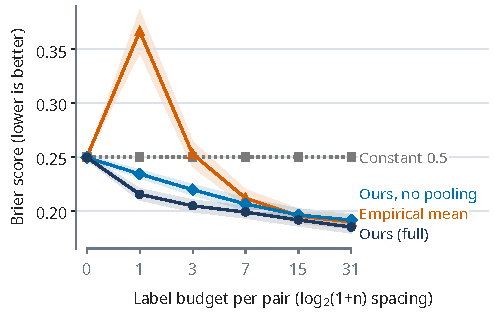
\includegraphics[width=0.62\linewidth]{figures/learning_curve.pdf}
  \caption{Mean Brier score per budget in the local replica; bands are $\pm 1.96$ standard errors over pairs (not clustered, for display only). The empirical mean is worse than a constant at budget 1, where a single label sets the prediction to 0 or 1.}
  \label{fig:curve}
\end{figure}

\paragraph{Main comparison.} Table~\ref{tab:main} and Figure~\ref{fig:curve} summarise the local replica. Our predictor improves on the constant by \DiffConst{} Brier ALC and on the official empirical-mean baseline by \DiffMean{}. It has the lower ALC on \WinConst\% of pairs against the constant and \WinMean\% against the empirical mean. Most of the gain is at budgets 1--7: at budget 1, where the empirical mean scores 0.367, our predictor scores 0.215. At budget 31 the two differ by about 0.005, as expected once a pair has enough labels of its own.

\paragraph{Where the gain comes from.} Pooling labels across subjects accounts for \DiffPool{} of ALC. Without pooling, the model still beats the empirical mean, because shrinkage and the probit correction keep single labels from producing extreme predictions. The offline subject ability adds no detectable gain: \DiffSubj{} with pooling and \DiffSubjNoPool{} without. This held although 80\% of simulated pairs matched a fitted ability at some key level (the rest fell back to the provider mean or the population). The fitted scales suggest why: the spread of $\lambda\theta_s$ (standard deviation 0.56 logits) is small next to the spread of benchmark intercepts (1.29) and of item effects (1.27), so knowing the subject moves predictions little, and once a few labels arrive $u_{sb}$ absorbs it.

\paragraph{Item effects.} With one shared split per benchmark, item effects are never identified for evaluation items; ALC is then \AlcOursShared{} and the pooling gain is \DiffPoolShared{}, close to the per-pair split. With at most eight subjects and 31 labels each on benchmarks of hundreds of items, a revealed item rarely recurs among another subject's evaluation items, so the gain from pooling comes from learning $c_b$, not $v_i$.

\paragraph{Sensitivity to the prior scales.} Table~\ref{tab:sens} halves and doubles each of $\sigma_c$, $\sigma_u$ and $\sigma_v$ with the others fixed. Halving $\sigma_c$ or $\sigma_u$ or doubling $\sigma_v$ costs 0.002--0.006 ALC; the other three changes gain at most 0.001, less than the spread across seeds below. Over-confident priors on the benchmark intercept and the subject deviation hurt more than vague ones. These runs share the folds and seed of the main run, so they show sensitivity, not out-of-sample tuning; we did not change the submitted scales after seeing them.

\begin{table}[t]
  \caption{Brier ALC of the full predictor when one prior scale is multiplied by 0.5 or 2 (local replica, same folds and seed as Table~\ref{tab:main}).}
  \label{tab:sens}
  \centering
  \small
  \begin{tabular}{lccc}
\toprule
Scale & $\times 0.5$ & $\times 1$ (submitted) & $\times 2$ \\
\midrule
$\sigma_c$ & 0.2098 & 0.2055 & 0.2047 \\
$\sigma_u$ & 0.2076 & 0.2055 & 0.2046 \\
$\sigma_v$ & 0.2049 & 0.2055 & 0.2110 \\
\bottomrule
\end{tabular}

\end{table}

\paragraph{Seeds.} Rerunning the replica with different fold assignments, subject samples, splits and label draws gave ALC \SeedRange{} over \NSeeds{} seeds for the full predictor.

\paragraph{Platform result.} \OnlineResult

\section{Exploratory: item difficulty from text (not in the submitted predictor)}
\label{sec:explore}

Budget 0 carries 10\% of the score, and item effects of evaluation items are never revealed, so information about an item before any label arrives would help at every budget. After submitting, we ran two experiments with the item text in measurement-db. Neither changes the submitted predictor; both enter Eq.~\ref{eq:model} as a fixed item offset $\beta(\ell_i - \bar\ell)$, where $\ell_i$ is a predicted log-odds of success for item $i$, and the offset also enters the fit of revealed labels.

\paragraph{Bag of words: negative.} A ridge regression from hashed word uni- and bigrams and simple format statistics (length, digits, answer options, code) of the item text to the item's pooled log-odds accuracy, trained on \TextBench{} training benchmarks with benchmark-grouped five-fold cross-validation, did not transfer to held-out benchmarks: the best out-of-fold item-level $R^2$ was \TextItemRtwo{} and the within-benchmark correlation \TextWithin{}. The features mostly identify the benchmark. With out-of-fold predictions and $\beta=0.5$ in the full replica, ALC changed by \TextAlcDiff{}.

\paragraph{LLM judgments: preliminary positive.} We asked an LLM (GPT-6-astra through the Codex command-line tool, 20 items per prompt) for the probability that ``a typical AI system evaluated on this benchmark'' answers each item, for 80 random items from each of \LlmBench{} held-out benchmarks. The judged log-odds correlate with the items' pooled log-odds accuracy at \LlmWithinCorr{} within a benchmark on average (from \LlmWithinMin{} to \LlmWithinMax{}) and at \LlmBenchCorr{} across the eight benchmark means. We reran the replica on these benchmarks, restricting evaluation items to the judged ones (\LlmPairs{} pairs), with $\bar\ell$ the mean judged log-odds (Table~\ref{tab:llm}). All three values of $\beta$ lower ALC, mostly at budget 0, but every interval is wide, $\beta$ was chosen on the same benchmarks, and one benchmark had a negative correlation. Asking for one item at a time, as a predictor would at scoring time, gave log-odds that correlate with the batch ones at \SingleCorrBatch{} (\SingleN{} items) but are more optimistic (mean \SingleMean{} against \SingleBatchMean{}), so the centring would have to be recalibrated. Using this at scoring time needs a paid API key and makes the predictor non-deterministic; a full test needs judgments for all evaluation items in the replica.

\begin{table}[t]
  \caption{Exploratory LLM item-difficulty offset (not submitted). Local replica restricted to \LlmItems{} judged items on \LlmBench{} held-out benchmarks (\LlmPairs{} pairs). Differences are paired, with 95\% cluster-bootstrap intervals over benchmarks.}
  \label{tab:llm}
  \centering
  \small
  \begin{tabular}{lcccc}
    \toprule
    Predictor & ALC & Difference & $B_0$ & $B_3$ \\
    \midrule
    Submitted (label-only) & \LlmAlcBase{} & -- & \LlmBzeroBase{} & \LlmBthreeBase{} \\
    \quad + LLM offset, $\beta=0.4$ & \LlmAlcFour{} & \LlmDiffFour{} & \LlmBzeroFour{} & \LlmBthreeFour{} \\
    \quad + LLM offset, $\beta=0.7$ & \LlmAlcSeven{} & \LlmDiffSeven{} & \LlmBzeroSeven{} & \LlmBthreeSeven{} \\
    \quad + LLM offset, $\beta=1.0$ & \LlmAlcTen{} & \LlmDiffTen{} & \LlmBzeroTen{} & \LlmBthreeTen{} \\
    \bottomrule
  \end{tabular}
\end{table}

\section{Limitations}
\label{sec:limits}

\begin{itemize}
  \item \textbf{Budget 0 is nearly uninformed.} $B_0$ is 0.249 against 0.250 for a constant. The predictor does not read item text, so it cannot tell a hard new benchmark from an easy one before labels arrive. An LLM-judged item offset looks promising in a small probe (\S\ref{sec:explore}) but was not submitted, because it needs an API key at scoring time and its evidence is still weak.
  \item \textbf{The local replica is our reading of the protocol.} The number of sampled subjects per benchmark, the split design and subject overlap between pools are unknown (\S\ref{sec:setup}). The training benchmarks may also differ from the private test pool. The local numbers rank methods under our assumptions; they do not predict the leaderboard score.
  \item \textbf{The subject prior failed to help} in our replica, and $\lambda$ comes from leave-one-benchmark-out cells that are dominated by benchmarks with many subjects. Our subject keys rely on exact matches of normalised names.
  \item \textbf{Approximations.} The Laplace variances are diagonal and ignore the negative posterior correlation between $c_b$ and $u_{sb}$, which overstates predictive variance somewhat. The hyperparameters are point estimates; $\sigma_v$ is estimated from item accuracy pooled over subjects, which mixes item difficulty with subject composition.
  \item \textbf{Scope of the evaluation.} One local seed was used for the ablations, sensitivity runs reuse the main run's folds, and the replica caps evaluation items at 150 per pair and subjects at eight per benchmark.
  \item \textbf{No acquisition policy.} We used random acquisition and did not test alternatives.
\end{itemize}

\paragraph{Data notes for the organisers.} Checking the training release one level down (revision \texttt{54074453}), we recomputed the catalogue counts of the 160 benchmarks listed as binary, item-level and public. Response and subject counts match for all 160 and item counts for 159; for \texttt{ceval} the catalogue lists 13{,}951 items while the response table has 1{,}346 distinct item IDs. Four of these benchmarks (\texttt{chartmuseum}, \texttt{ineqmath}, \texttt{mmmu\_dev\_val}, \texttt{naturalreasoning}) contain only missing responses, and 46 others contain some missing responses; our pipeline drops missing values. The per-benchmark table is released with the code.

\section{Reproducibility}

Code, the fitted prior and the scripts for every number in this report are released at \url{https://github.com/ting-hong-shieh/paiec-hierarchical-bayes} (MIT licence). From the repository root:
\begin{enumerate}
  \item download the binary item-level tables of measurement-db (revision \texttt{54074453}) with \texttt{tools/download\_measurement\_db.py};
  \item \texttt{python tools/build\_tables.py --cache <cache> --out data/};
  \item \texttt{python tools/fit\_prior.py --data data/ --out submission/prior.json};
  \item \texttt{python tools/simulate.py --data data/ --out results/sim\_per\_pair.json} (add \texttt{--split shared}, \texttt{--seed}, \texttt{--scale-sc} etc.\ for the other runs);
  \item \texttt{python tools/analyze.py} to regenerate the tables and the figure;
  \item zip \texttt{submission/} (model.py, prior.json, README.md) and check it with the official \texttt{check\_submission\_zip.py}.
\end{enumerate}
Each simulation takes about three minutes on a 24-thread CPU and about 4\,GB of memory. The exploratory runs use \texttt{tools/download\_items.py}, \texttt{tools/text\_prior.py}, \texttt{tools/llm\_probe.py} and \texttt{simulate.py --model experiments/model\_with\_offset.py --text-beta} (with \texttt{--text-oof} or \texttt{--llm-probe}). The submitted predictor itself is deterministic and makes no network calls.

\section*{Disclosures}

\textbf{Training data.} Only the AI Measurement Data Bank \citep{measurementdb2026}, revision \texttt{54074453}, as listed in the competition's benchmark inventory: tables \texttt{benchmarks}, \texttt{subjects} and \texttt{responses} (and \texttt{items} for \S\ref{sec:explore}) of benchmarks with binary, item-level, public responses. The submitted predictor uses no item text, traces or embeddings; the exploratory experiments of \S\ref{sec:explore} also use the item text in the \texttt{items} tables. \textbf{Pretrained models.} None in the submitted predictor; GPT-6-astra, through the Codex command-line tool, produced the item judgments of the exploratory probe. \textbf{Coding assistant.} The code and a first draft of this report were written with an LLM coding assistant (Claude Code, Anthropic) under the author's direction; the author checked the method, the numbers and the text. \textbf{Prior work reused.} The official baseline repository \citep{paiec_baselines_2026} was used for its submission checker and as the empirical-mean comparison.

\bibliographystyle{plainnat}
\bibliography{refs}

\end{document}
